\beginsong{Nachts steht Hunger starr}[
    wuw={olka (Erich Scholz), 
    Nerother Wandervogel}, 
    jahr={1934}, 
    pfii={120}, 
    pfiii={61}, 
    siru={168},
]

\beginverse
\endverse 
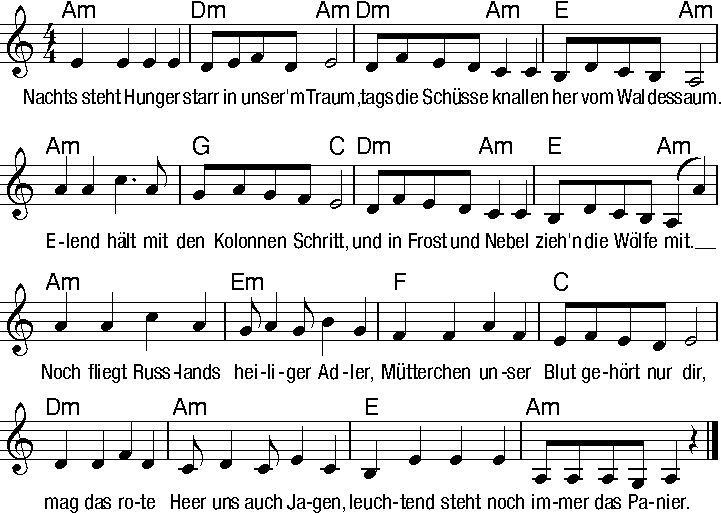
\includegraphics[draft=false, width=1\textwidth]{Noten/Lied068.pdf}	

\beginverse
\[Am]Ach, dahin ist \[Dm]eine stolze \[Am]Macht,
\[Dm]keine Glocken \[Am]klingen \[E]durch die rote \[Am]Nacht.
\[Am]Postenschritte, \[G]keine Freiheit \[C]mehr,
\[Dm]hinter Stachel\[Am]draht steht \[E]stumm ein müdes \[Am]Heer.
\[Am]Einer singt die \[Em]alten Lieder,
\[F]lockt uns Schwermut und \[C]Sehnsucht aus der Brust,
\[Dm]wild und trotzig \[Am]klingt es wieder,
\[E]im Vergess'nen \[Am]liegt die alte Lust.
\endverse

\beginchorus
\lrep \[Am]Noch fliegt Russlands \[Em]heiliger Adler,
\[F]Mütterchen, unser \[C]Blut gehört nur dir,
\[Dm]mag das rote \[Am]Heer uns auch jagen,
\[E]leuchtend steht noch \[Am]immer das Panier. \rrep
\endchorus

\beginverse
^Und als Heer, das ^keine Heimat ^hat,
^zieh'n wir ausge^wiesen ^nun von Stadt zu ^Stadt.
^Menschen kommen, ^hören unser ^Lied,
^weiter geht die ^Fahrt, der ^Ruhm uns sinnlos ^blüht.
''^Heimat, Heimat!'', ^summen die Chöre,
^tausendfältig ent^steht uns neu dein Bild.
^Glockenläuten, ^uns're Tenöre,
^Orgelbässe ^klingen dumpf und wild.
\endverse

\printchorus

\endsong

\beginscripture{}
Kosaken = Gemeinschaften freier Reiterverbände, zu denen sich flüchtige Russen und Ukrainer, manchmal auch nur Abenteurer oder anderweitig Abtrünnige, in den südlichen Steppengebieten zusammenschlossen;
Das Lied versetzt in die Lage ''weißer'' Kosaken, die durch den Sieg der kommunistischen Revolution ihre russische Heimat verloren und sich in der Fremde singend ihren Lebensunterhalt verdienen müssen. Als Sänger aber auch als Opfer eines brutalen Regimes boten sie sich besonders nach 1933 vielen Bündischen zur Identifikation an.
\endscripture
